\documentclass{template}
\usepackage{color}
\usepackage[hyphens]{url}
\usepackage{longtable}
\usepackage{graphicx}
\usepackage{enumitem}
\usepackage{pdfpages}
\usepackage{hyperref}

\def\etal{{\it et al.~}}
\newenvironment{packed_enum}{
\begin{enumerate}
  \setlength{\itemsep}{1pt}
  \setlength{\parskip}{0pt}
  \setlength{\parsep}{0pt}
}{\end{enumerate}}
\newenvironment{packed_item}{
\begin{itemize}
  \setlength{\itemsep}{1pt}
  \setlength{\parskip}{0pt}
  \setlength{\parsep}{0pt}
}{\end{itemize}}

\begin{document}

\title{Tor's Usability for Censorship Circumvention}
\numberofauthors{1}
\author{
 \alignauthor Linda N. Lee, David Fifield, Nathan Malkin \\
   \vspace{0.5em}
   \affaddr{University of California, Berkeley} \\
   \affaddr{\{lnl,fifield,nmalkin\}@cs.berkeley.edu}\\
}
\maketitle

\begin{abstract}
Tor has grown beyond its original purpose as an anonymity tool and has 
since become an important censorship circumvention tool. {\color {red} cite something here..}
We specifically examine its usability as a censorship circumvention tool,
an essential facet for adoption and use.  
We focus our analysis on the connection configuration interface of Tor browser,
as censorship circumvention requires correct transport configurations.
We will conduct a large-scale user study examining 60-100 of users 
on how they navigate Tor's configuration wizard to complete seven browsing tasks 
in three different adversarial settings. Our study combines quantitative measurements (interface
paths taken to success, time to success, and which configuration was chosen) and
qualitative measurements (if users were comfortable with use, what was most confusing, and 
if they would use the browser again). The first phase of the study will evaluate if and how 
easily users can circumvent censorship using Tor Browser. The second phase
of the study will test improvements to the interface and an alternate interface. 
Our goal is to integrate positive usability changes into the Tor Browser. Since
the configuration interface is modular and does not require changes to the Tor Browser
functionality, these changes will be easy to deploy. 

\end{abstract}

\keywords{Censorship, Security, User Studies, Anonymity, Tor}

\section{Tor's Usability}
As the most widely used anonymity tool today, Tor is primarily known as an anonymity tool. 
For this reason, user studies on Tor have been solely about, the usability of Tor as an 
anonymity tool. Norcie~\cite{norcie2012eliminating} conducted an experiment which identified 
``stopping points'' in Tor browser,  documenting points when people would get frustrated enough 
to stop using Tor. To our knowledge, that has been the only published user study of Tor. 
Since then, Tor has had a lot of updates.There have been been no published usability evaluations of
Tor Browser since the introduction of the 4.0 series, which introduced radical UI changes. 
Lee and Fifield \cite {uxsprint} ran a small pilot study testing the download, install, and user interface of Tor Browser. 
This study uncovered a number of bugs and stopping points. Changes made are reflected in series 
5.1 and later. 

There are still many features of Tor that are left unevaluated through user research---such as advanced web tasks (such as accessing hidden services), the configuration menu to connect to the Tor network, configuring for automatic updates, and identity/cookie management. Rather than selecting the features to study in isolation, 
we decided to focus on an important use case of Tor browser, censorship circumvention. 
Internet censorship is shown to be pervasive across the world today \ref{faris2008measuring}. 
To our knowledge, this is the first user study investigating the usability of Tor as a 
censorship circumvention tool, rather than an anonymity tool.

\section{Design}

\noindent {\bfseries Overview}
There is a configuration interface (Figure ~\ref{fig:interface}) to help guide users through 
setting up their connection to the Tor network. Through this, users can configure Tor to set up a bridge,
proxy, or both. Since proxies are not a Tor-specific notion nor explicitly required to circumvent censorship, 
we will focus our study on bridge configuration. We accomplish this by placing users in crafted simulated 
censorship environments which require particular bridge configurations to circumvent censorship. 

Our hypothesis is that the average user does not have knowledge
knowledge on how certain pluggable transports work, or to provide non-publicly listed IP
addresses bridges. Certain real-world censorship settings require the user to provide this
information during configuration, which will affect how successful users are at 
circumventing censorship using Tor. Participants may receive additional information through word 
of mouth, help from relatives, or blogs. Our study will measure if the configuration
interface successfully guides users to correctly configuring their browser, not accounting 
for any additional  information that a real user may have.\\

\begin{figure*}[t]
\label{fig:interface}
  \centering
    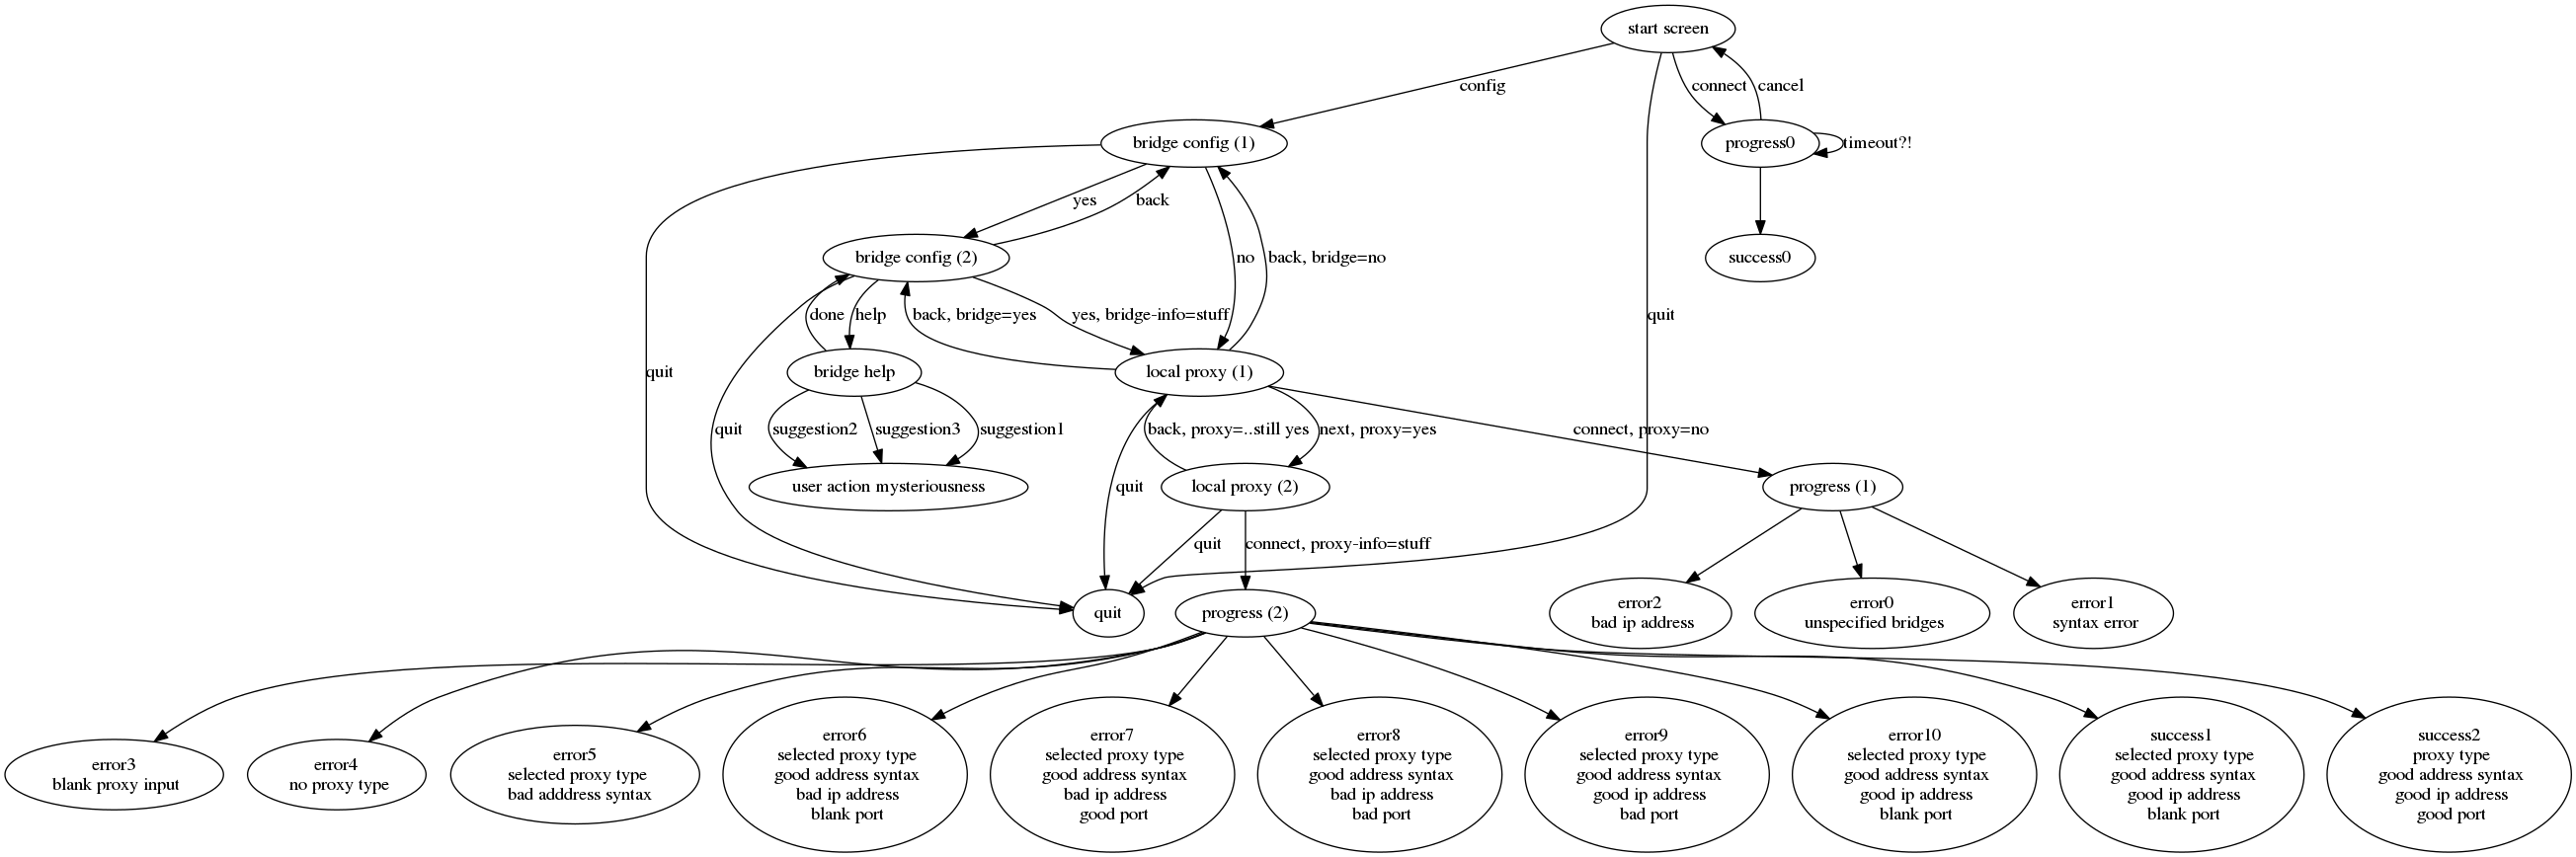
\includegraphics[width=\textwidth]{../torconfig.png}
    \caption{This flow chart shows all of the possible paths taken through the
    Tor configuration interface. A state represents a window in the interface,
    with the exception of the leaves, which indicate the final action taken by
    the interface (``q'' for quit, ``s'' for success, and ``e'' for error). The
    transitions between the states indicate which user action causes that
    transition. The cause for error is can be found
\href{https://github.com/lindanlee/circumvention-ux-tor/blob/master/torconfig.dot}{here}.}
\end{figure*}

\begin{figure}[t]
\label{fig:bridges}
  \centering
    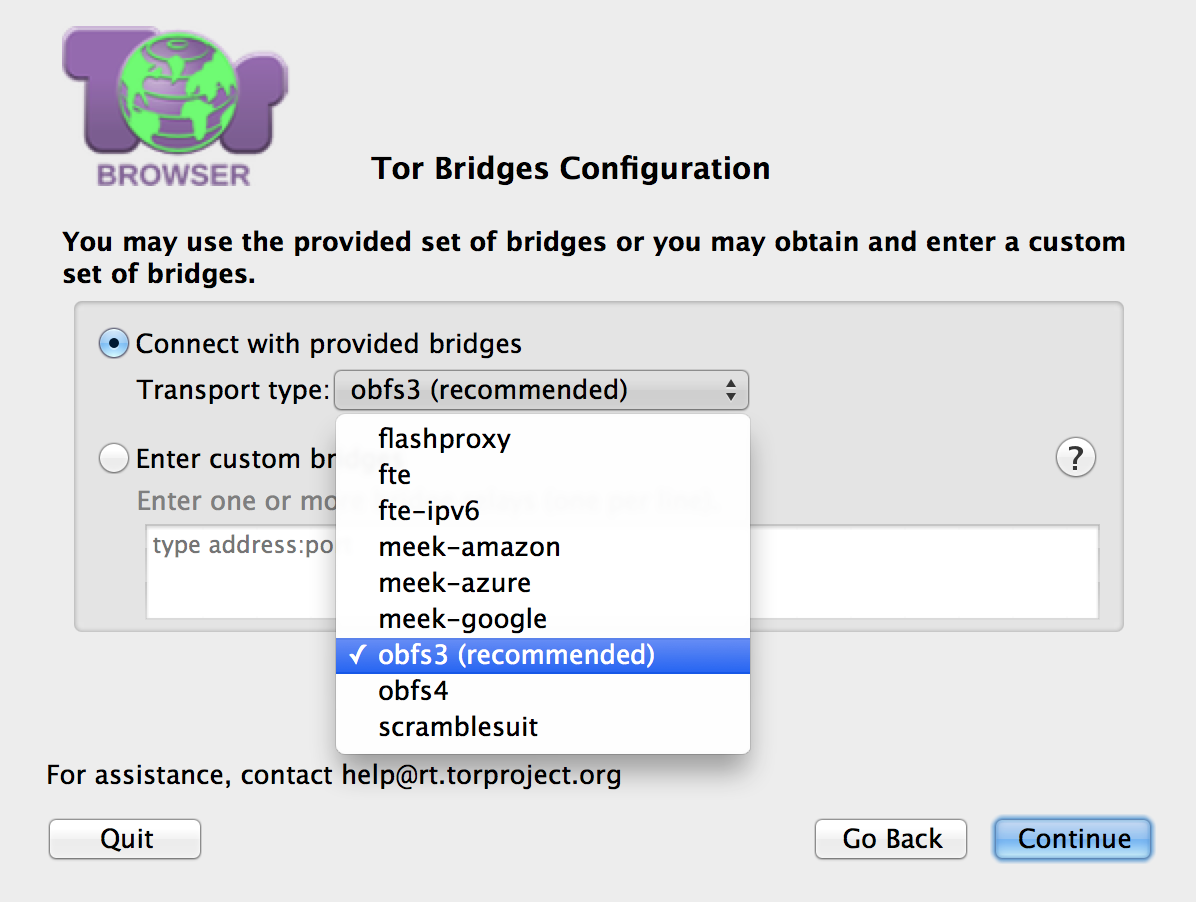
\includegraphics[width=0.5\textwidth]{configuration-screenshot.png}
    \caption{The Tor Bridges Configuration window of the Tor configuration
    interface. Tor users in censored environments and some of our participants
    will be required to select the correct bridge for circumventing censorship.
    Note that the interface prompts users to choose a transport type, which can be
    the source of confusion. Bridges are non-listed guard relays to the Tor
    network, and some of them can have transport types which obfuscate traffic in
    different ways.}
\end{figure}


\noindent {\bfseries Experiment Logistics} 
The IRB protocol to run this user study has been approved (2014-12-6995). 
We plan to recruit from 100-200 users for the purpose of this study, 
making it the largest user study of Tor to date.  This study will be conducted at the
Experimental Social Science Laboratory (Xlab)
at the University of California, Berkeley, which consists of 36 laptops,
separated by cubicle walls. We will use individual host firewalls to simulate
censorship environments and will record computer screens to capture 
user activity. The total length of the experiment, including briefing, completing the censorship 
circumvention tasks, exit survey, and debriefing, will be about an hour.
Participants will be compensated \$30 for their time, which covers
minimum wage for an hour and any transportation costs to the lab.  \\

\noindent {\bfseries Experiment Flow} 
We will run three sets of the experiment, the first set to test the current configuration
interface, a second set to test the improved interface, and a third set to test the 
alternate configuration interface. The experiment flow will be the same across all 
sets of experiments, with the fact that the configuration interface will be altered 
across sets. 

The experiment begins with the participants being informed that they are in a
simulated censorship
environment, where some --- but not all --- websites are blocked. We will
instruct them to visit a non-blocked website and a blocked website on a
``standard'' browser (one that is not used for censorship circumvention, such
as Chrome, Safari, or Firefox) to illustrate the situation.
Then, the participants will find out the role they they will be playing in the study.
This role is that of a regular citizen, who is trying to visit blocked websites
for non-critical leisurely purposes,
and that there is a minimal chance of risk. This information is given
to achieve
consistency across participants: their behavior might be different if they were
visiting websites to accomplish a critical task, or if they knew that there
were great risks. 

After explaining the situation and their role, we will explain what Tor is, and
how they can use it if necessary, and instruct them to complete a set of
tasks which will require visiting blocked websites. Ultimately, the
participants will need to configure their Tor Browser to circumvent the
simulated censorship environment. These tasks have a three-fold purpose of
providing participants with feedback (if they did not correctly configure their
browser, they cannot reach the website),  motivating the participants to
configure the browser correctly, and providing the researchers with an
indicator of successful censorship circumvention.
Participants' screens will be recorded to capture how they configure
their browser, and to provide additional evidence that they have completed the
tasks.

After users complete the browsing tasks, we will administer a survey that 1)
measures demographics, technical fluency, and
familiarity with Tor and 2) collects qualitative feedback from
participants about their browsing experience as a whole
and the configuration interface specifically.
A rough draft of the survey can be
found
\href{http://www.surveygizmo.com/collab/2085559/Tor-Usability-Survey}{here}.

The experiment will conclude with a debriefing, which will inform that the
participants of their screen capture and obtaining re-consent for the
information.  \\

\noindent {\bfseries Censorship Environment Simulation} 
We plan to simulate three censorship environments.
They are informed by our experience with pluggable transports
and knowledge of commonly seen censorship techniques.
They are not meant perfectly to replicate the network environment
in any particular country. Although inspired by reality, these
abstract simulations are intended to require distinct configurations
of the Tor Browser from our participants. 

\begin{itemize} \itemsep1pt \parskip0pt \parsep0pt
\item {\bfseries Mild censorship} 
(Reflective of countries such as {\color{red}?? and ??}.)
Certain domain names are blocked. Reaching these 
domains requires any use of a censorship circumvention 
tool. The default option to ``connect'' to the Tor network 
directly will circumvent this censor. Additional correct
bridge or proxy configuration are optional. 
\item {\bfseries Intermediate censorship} 
(Reflective of countries such as {\color{red}?? and ??}.)
Certain domain names are blocked. Censorship circumvention
tools are blocked. Since Tor is blocked by blocking all public Tor
relay nodes, the default option to ``connect'' to the Tor network
directly will fail. A choice of a hard-coded bridge (see Figure ~\ref{fig:bridges})
or a valid non-public bridge is required to circumvent this censor.  
Additional correct proxy configuration is optional.
\item {\bfseries Comprehensive censorship} 
(Reflective of countries such as China and Syria.)
Certain domain names are blocked. Censorship circumvention tools
are thoroughly blocked. Tor is blocked by blocking all public
Tor relay nodes, and the censor has examined source code to block
all hard-coded bridge relays in the configuration interface. The default option
to ``connect'' to the Tor network directly will fail. Choosing any bridges other than
``meek-amazon,'' ``meek-azure,'' and``meek-google,'' will fail. This is because 
domain-fronting requires censors to block entire CDNs to also block this
transport (which will cause huge collateral blocking damage), making it resistant to agressive censorship environments.
(See ~\cite{fifield2015blocking} for additional details.)\\
\end{itemize}

\noindent {\bfseries List of Tasks} 
In our experimental setup, successful completion of 
these given tasks requires of correct configuration.
The difficulty of circumventing  censorship to visit the 
websites required for the tasks will vary depending on the 
simulated censorship environment. Since all participants will be given the 
same set of tasks, regardless of the censorship environment, 
the difficulty of completing the tasks remains constant assuming
correct configuration. The tasks themselves are not intended to
be challenging.

The tasks were initially inspired by the top Alexa sites, 
an indication of representative and relevant browsing behavior. 
From these, we selected sites which were commonly censored, 
but filtered tasks that would require a participant to reveal private information 
(such as login information) for ethical considerations. These tasks
were further refined after performing a pilot study of the experiment. 
We hope the tasks convey an example of how of a user might 
browse the Internet in a censored environment. 

\begin{itemize} \itemsep1pt \parskip0pt \parsep0pt
\item Google search for the population of Zimbabwe. 
\item On YouTube, find a video playing Bach's ``Ode to Joy.''
\item Find the Amazon best-sellers in ``Movies \& TV.''
\item On Yahoo, find the exchange rate of Dollars to Euros.
\item Find the Wikipedia ``History'' portal's featured article. 
\item On Twitter, find the currently trending topics.
\item On Bing Maps, find directions from Times Square to Carnegie Hall.
\end{itemize}

\section{What we hope to accomplish}

We plan to finish the user study by the end of the semester. 
From this experiment, we hope to accomplish the following: 

\begin{itemize} \itemsep1pt \parskip0pt \parsep0pt
\item {\bfseries Test the Tor configuration interface} We will perform the largest-scale user study 
of Tor to date, measuring how users configure Tor in three different adversarial settings. 
\item {\bfseries Test an improved configuration interface} With the measurements collected
from testing the interface as-is, we will be designing ways to improve the interface to minimize
time taken, paths taken, and error states reached.
\item {\bfseries Test an alternative configuration interface} A Tor developer has offered
to design a mock-up interface for an alternative configuration interface which will
greatly automate the process. There are tradeoffs between ease of use and transparency
of the systems, and ethical considerations with loggable errors resulting from automated configuration. 
\item {\bfseries Push changes} We have the support of Tor developers
to improve this interface. Additionally, since the configuration interface does not require 
any changes to the Tor Browser functionality, improvements to the interface will
be easy to deploy. 
\end{itemize}

\section{Resources}
\noindent Our online artifacts of the work done during this class, Fall 2015,
are below: 
\begin{itemize} \itemsep1pt \parskip0pt \parsep0pt
\item \href{https://github.com/lindanlee/circumvention-ux-tor}{github repo with experiment plans, code, and paper}
\item \href {https://github.com/lindanlee/circumvention-ux-tor/blob/master/pilot/1-strict.mp4}{pilot video 1}
	\href{https://github.com/lindanlee/circumvention-ux-tor/blob/master/pilot/2-lax.mp4}{pilot video 2}
\item \href{https://github.com/lindanlee/circumvention-ux-tor/blob/master/setup/setup-environment}{experimental setup code: firewall and screen capture} 
\item \href{https://github.com/lindanlee/circumvention-ux-tor/blob/master/setup/takedown-environment}{experimental takedown code: saving files and cleanup} 
\end{itemize}

% from anonymity study
Our online artifacts of study of Tor as an anonymity tool, such as 
the summary, results, and resulting browser changes are below:
\begin{itemize} \itemsep1pt \parskip0pt \parsep0pt
\item \href{https://trac.torproject.org/projects/tor/wiki/org/meetings/2015UXsprint}{blog post summary}
\item \href{https://blog.torproject.org/blog/ux-sprint-2015-wrapup}{changes made to Tor}
\item \href{https://people.torproject.org/~dcf/uxsprint2015/}{subtitled screen videos}
\end{itemize}

\bibliographystyle{abbrv}
\bibliography{circumvention-experiment.bib} 
\end{document}
